\section{Cylinders and Quadric Surfaces}
\begin{definition}[Traces]
    A trace of a surface is the curve of its intersection with a coordinate plane.
\end{definition}
\begin{definition}[Cylinder]
    A surface consisting of all lines parallel to it that pass through a given plane curve.
\end{definition}
\begin{definition}[Quadric Surface]
    A surface defined by a polynomial equation of degree 2, that is an equation of the form
    \[
        Ax^2+By^2+Cz^2+Dxy+Eyz+Fxz+Gx+Hy+Iz+J=0,\; A,B,C,D,E,F,G,H,I,J\in\R
    \]
\end{definition}
Basic quadric surfaces can be defined of the forms
\begin{itemize}
    \item \(z=Ax^2 +By^2\) describes a paraboloid
    \item \(z^2 =Ax^2 + By^2\) describes a double cone 
    \item \(\frac{x^2}{A^2}+\frac{y^2}{B^2}-\frac{z^2}{C^2}=1\) describes a hyperboloid of one sheet
    \item \(-\frac{x^2}{A^2}-\frac{y^2}{B^2}+\frac{z^2}{C^2}=1\) describes a hyperboloid of two sheets
    \item \(\frac{x^2}{A^2}+\frac{y^2}{B^2}+\frac{z^2}{C^2}=1\) descibes an elipsoid
\end{itemize}
\newpage
\chapter{Vector Functions}
\section{Vector Functions and Space Curves}
\begin{definition}[Vector-Valued Function]
    A vector-valued function \(\vec{r}:\R\to\R^n\) has a domain of real numbers and a range of vectors.
\end{definition}
\begin{definition}[Component Functions]
    Component functions \(f,g,h\) of a vector function \(\vec{r}\) are given as
    \[
        \vec{r}(t)=f(t)\ihat+g(t)\jhat+h(t)\hatk
    \]
\end{definition}
\begin{definition}[Space Curve]
    A space curve is the set \(C\) of points \((x,y,z)\) where
    \[
        C=\{(x,y,z)\mid t\in I \subseteq \R,x=f(t),y=g(t),z=h(t)\}
    \]
\end{definition}
Let \(\vec{r}(t)\langle 1+3t,2-4t,7+t \rangle\). It follows that
\[
    \langle x,y,z \rangle = \langle 1+3t,2-4t,7+t \rangle 
\]
\[
    \Rightarrow x=1+3t,\quad y=2-4t,\quad z=7+t
\]
These are the \textbf{parametric equations} of this vector function. We can then also show that
\[
    t=\frac{x-1}{3}=\frac{y-2}{-4}=z-7
\]
These are the \textbf{symmetric equations} of this vector function.
\begin{center}
    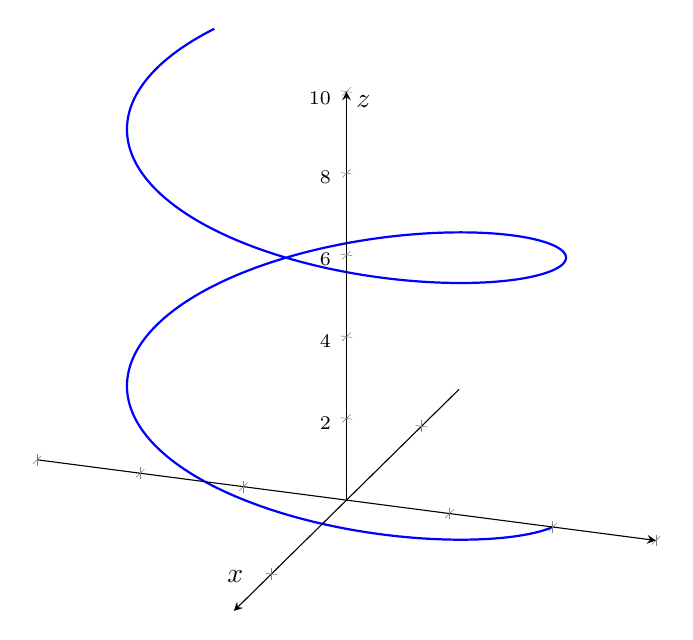
\begin{tikzpicture}
        \begin{axis}[
            width=2*175pt,
			tick label style={font=\scriptsize},
			axis on top,
			view={110}{30},
			axis lines=center,
			name=3dplot,
			ymin=-1.5, ymax=1.5, xmin=-1.5, xmax=1.5, zmin=0, zmax=10,
			xlabel=$x$, ylabel=, zlabel=$z$,
            xticklabel=\empty,yticklabel=\empty]
            \addplot3[samples=600, samples y=0, domain=0:10, domain y=0:10, color=blue, thick] ({sin(deg(x))},{cos(deg(x))},{x});
        \end{axis}
    \end{tikzpicture}
    \[
        \vec{r}(t)=\sin(t)\hati+\cos(t)\hatj+t\hatk,\; t\in\R^+\cup\{0\}
    \]
\end{center}
\begin{definition}[Limit of a Vector Function]
    If \(\vec{r}(t)= \langle f(t),g(t),h(t) \rangle \), then we will have
    \[
        \lim_{t\to a}\vec{r}(t)=\lim_{t\to a}\langle f(t),g(t),h(t) \rangle  = \langle \lim_{t\to a}f(t),\lim_{t\to a}g(t),\lim_{t\to a}h(t)    \rangle 
    \]
    provided the limits of the component functions exist.
\end{definition}